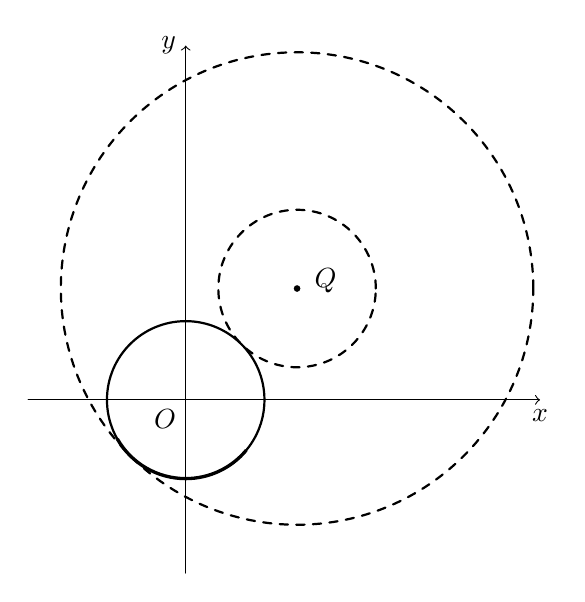
\begin{tikzpicture}[line cap=round,line join=round,scale=1]
\usetikzlibrary{calc}

% axes
\draw[->] (-2.0,0) -- (4.5,0) node[below] {$x$};
\draw[->] (0,-2.2) -- (0,4.5) node[left] {$y$};

% key points
\coordinate (O) at (0,0);
\coordinate (Q) at ({sqrt(2)},{sqrt(2)});

\node[below left] at (O) {$O$};
\fill (Q) circle (1.2pt);
\node[right] at ($(Q)+(0.1,0.1)$) {$Q$};

% circle C: x^2 + y^2 = 1
\draw[thick] (O) circle (1);

% annulus boundaries centered at Q: radii 1 and 3 (dashed)
\draw[dashed,thick] (Q) circle (1);
\draw[dashed,thick] (Q) circle (3);

% small arc highlight on circle C (schematic, like the picture)
\draw[very thick] (O) ++(210:1) arc[start angle=210,end angle=320,radius=1];

\end{tikzpicture}